% main.tex

\documentclass[a4paper,12pt,oneside,openany,headsepline,bibliography=totocnumbered]{scrbook}

% Import settings, packages, etc.
% List of packages and settings

\usepackage[T1]{fontenc}
\usepackage[utf8]{inputenc}
\usepackage{graphicx}
\usepackage{epstopdf}
\usepackage{amsmath}
\usepackage{amssymb}
\usepackage{amsfonts}
\usepackage{eucal}
\usepackage{fancyhdr}
\usepackage{url}
\usepackage{listings}
\usepackage[printonlyused]{acronym}
\usepackage{algorithmic}
\usepackage{algorithm}
\usepackage{multicol}
\usepackage{hyphenat}

% Set graphics path
\graphicspath{{../figures/}}

% URL style
\urlstyle{tt}

% Separation between list items
\setlength{\itemsep}{0ex plus0.2ex}

% Fancy headers
\setlength{\headsep}{8mm}
\pagestyle{fancyplain}
\renewcommand{\chaptermark}[1]{\markboth{#1}{#1}}
\renewcommand{\sectionmark}[1]{\markright{\thesection\ #1}}
\lhead[\fancyplain{}{\thepage}]{\fancyplain{}{\slshape \rightmark}}
\rhead[\fancyplain{}{\slshape \leftmark}]{\fancyplain{}{\thepage}}
\cfoot{}


\begin{document}

% Import frontpage
% Frontpage

\frontmatter

\begin{titlepage}
    \enlargethispage{3cm}
    \vspace*{-32mm}\hspace*{120mm}
    \includegraphics[scale=1.0]{rub_logo-eps-converted-to.pdf}
    
    \vspace*{11cm}\hspace*{0mm}
    \begin{minipage}[b]{1\linewidth}
        \sffamily
        \hspace{-17.2mm}\includegraphics[scale=1.0]{rub_slogan-eps-converted-to.pdf}\\
        
        \nohyphens{
            {\bfseries \LARGE \sffamily {\thtitle}}
        }\\
        
        \large{
            \thauthor
        }\\
        
        \vspace*{35mm}
        \normalsize{
            Seminar Paper\\
            \today\\
            Chair for Security Engineering - Prof. Dr.-Ing. Tim G{\"u}neysu\\
            Advisor: Georg Land
        }
    \end{minipage}
\end{titlepage}

\newpage\thispagestyle{empty}


% Abstract
\section*{Abstract}
\thispagestyle{abstract}

The imminent threat posed by quantum computing necessitates the transition to quantum-resistant cryptographic schemes like CRYSTALS-Dilithium, a leading lattice-based digital signature algorithm selected for standardization. Ensuring the feasibility and performance of side-channel resistant implementations of such schemes on embedded devices is a critical challenge. This paper introduces the most important aspects affecting the feasibility and performance of side-channel resistant implementations of post-quantum schemes, focusing on masking techniques, security levels (masking orders), performance metrics (execution time, cycle counts), implementation strategies, and the trade-offs between security and efficiency. We analyze, visualize, and compare all existing masked implementations of Dilithium regarding these aspects, providing a comprehensive discussion of their approaches. Our comparative study highlights how different implementations address the balance between security and performance, offering insights into optimal strategies for deploying secure and efficient post-quantum cryptography in resource-constrained environments. We emphasize the significance of refined sensitivity analyses, optimized masking gadgets, and the advantages of randomized signing in achieving practical side-channel resistance. Our findings serve as a guide for practitioners and researchers aiming to enhance the side-channel resistance of post-quantum cryptographic implementations without compromising practicality.


% Table of contents
\tableofcontents
\thispagestyle{contents}

\chapter*{Acronyms}
\thispagestyle{acronyms}
\addcontentsline{toc}{chapter}{Acronyms}
\begin{acronym}[PQC]
    \acro{ARM}{Advanced RISC Machine}
    \acro{B2A}{Boolean-to-Arithmetic}
    \acro{DPA}{Differential Power Analysis}
    \acro{ECC}{Elliptic Curve Cryptography}
    \acro{MLWE}{Module Learning withs Errors}
    \acro{NIST}{National Institute of Standards and Technology}
    \acro{NTT}{Number Theoretic Transform}
    \acro{PINI}{Probe-Isolating Non-Interference}
    \acro{PQC}{Post-Quantum Cryptography}
    \acro{SCA}{Side-Channel Attack}
    \acro{SPA}{Simple Power Analysis}
\end{acronym}


% Include all chapters as .tex files
% introduction.tex

\chapter{Introduction}
\thispagestyle{chapterstart}

\section{Motivation}

The rapid advancement of quantum computing technology poses a significant threat to current cryptographic systems, particularly those based on integer factorization and discrete logarithm problems, such as RSA and \ac{ECC}. Quantum algorithms like Shor's algorithm can solve these problems efficiently, rendering classical cryptosystems insecure. To address this threat, the \ac{NIST} initiated a standardization process for \ac{PQC} algorithms that are secure against both quantum and classical attacks.

Among the winning candidates in this process is the lattice-based scheme CRYSTALS-Dilithium, known for its strong security foundations and efficient performance. However, while Dilithium is resistant to quantum attacks, its implementations on embedded devices are vulnerable to \acp{SCA}, which exploit physical leakages to extract sensitive information.

Side-channel resistance is critical for embedded devices, often with limited resources and physical accessibility. Enhancing the side-channel resistance of Dilithium implementations is essential for securing future cryptographic systems in the quantum era.

\section{Goals}

The primary goal of this paper is to analyze and compare various side-channel resistant implementations of the Dilithium digital signature scheme, focusing on methodologies, security levels, performance, and feasibility on embedded devices. Specifically, the objectives are:

\begin{itemize}
    \item \textbf{In-depth Analysis}: Examine selected implementations, highlighting techniques used for security and performance improvements.
    \item \textbf{Comparative Evaluation}: Compare implementations in terms of security levels (masking orders), performance metrics, and practical considerations.
    \item \textbf{Discussion of Trade-offs}: Identify and discuss trade-offs between security and performance in different masking techniques.
    \item \textbf{Insights for Deployment}: Offer strategies for deploying secure and efficient Dilithium implementations in resource-constrained environments.
\end{itemize}

By achieving these goals, this paper aims to contribute to understanding side-channel resistant implementations of Dilithium and guide future research.

\section{Structure of the Paper}

This paper is structured as follows:

\begin{itemize}
    \item \textbf{Chapter 2 - Background}: Provides an overview of post-quantum cryptography and quantum threats, introduces side-channel attacks, and discusses masking techniques relevant to Dilithium.
    \item \textbf{Chapter 3 - Analysis}: Presents an in-depth analysis of selected side-channel resistant implementations of Dilithium, examining methodologies and practical considerations.
    \item \textbf{Chapter 4 - Comparative Analysis}: Compares the analyzed implementations, highlighting strengths and weaknesses, discussing trade-offs, and implications for deployment.
    \item \textbf{Chapter 5 - Conclusion}: Summarizes the findings, discusses implications for deploying side-channel resistant Dilithium implementations, and suggests directions for future research.
\end{itemize}

By following this structure, the paper builds from foundational concepts to detailed analysis and comparison, culminating in conclusions that inform both academic and practical perspectives.

\chapter{Background}
\thispagestyle{chapterstart}

\section{Post-Quantum Cryptography and Quantum Threats}

Post-Quantum Cryptography (\ac{PQC}) refers to cryptographic algorithms designed to withstand attacks from quantum computers, which pose a threat to conventional cryptosystems such as RSA and elliptic curve cryptography due to Shor’s algorithm. In response, the \ac{NIST} initiated a standardization process to evaluate and select quantum-resistant algorithms. The primary goal is to develop algorithms that are secure against both classical and quantum adversaries, without compromising efficiency on classical computing architectures. Lattice-based schemes, particularly \acp{KEM} like Kyber and signature schemes like Dilithium, have emerged as leading candidates due to their strong security foundations and favorable performance metrics \cite{Azouaoui22}.

\section{Side-Channel Attacks}

Side-channel attacks (\acp{SCA}) exploit physical leakages from cryptographic operations—such as timing, power consumption, and electromagnetic emissions—to extract sensitive information. These attacks are particularly effective on embedded devices, where physical access often allows attackers to measure leakage directly. \acp{SCA} are typically classified by the type of information they exploit:

\begin{itemize}
    \item \textbf{Timing Attacks:} Exploiting variations in the time taken by cryptographic operations.
    \item \textbf{Power Analysis:} Utilizing power consumption patterns to infer cryptographic keys or other sensitive information.
    \item \textbf{Electromagnetic Analysis:} Measuring electromagnetic radiation emitted during computation to uncover internal states.
\end{itemize}

In the context of \ac{PQC}, lattice-based cryptographic schemes present unique challenges for \ac{SCA} resistance. These schemes often involve complex arithmetic operations, such as polynomial multiplications and modular reductions, which are susceptible to \acp{SCA}. Research has shown that unmasked implementations of Kyber and Dilithium are vulnerable to \ac{DPA} and \ac{SPA}, particularly during the generation and manipulation of secret-dependent values \cite{Bos21}.

\section{Side-Channel Countermeasures}

Several countermeasures have been developed to mitigate side-channel threats in \ac{PQC} implementations, particularly for lattice-based schemes:

\begin{itemize}
    \item \textbf{Masking:} Masking is a technique where sensitive variables are split into several shares to prevent leakage of secret information. In lattice-based schemes, masking can be Boolean, arithmetic, or a combination, depending on the nature of the operations. For instance, Migliore et al.\ (2019) \cite{Migliore19} demonstrated that Boolean masking is effective for Dilithium, reducing leakage during sensitive polynomial operations. However, this approach incurs computational overhead, especially at higher security orders.
    \item \textbf{Bitslicing:} Bitslicing optimizes masking by arranging data in a format that allows parallel bitwise operations, reducing computational costs. Bronchain and Cassiers (2022) \cite{Bronchain22} applied bitslicing to efficiently manage Boolean and arithmetic masking conversions in lattice-based \acp{KEM}, achieving significant performance gains on the \ac{ARM} Cortex-M4 processor.
    \item \textbf{Improved Masking Gadgets:} High-order masking gadgets, such as those proposed by Coron et al.\ (2023) \cite{Coron23}, introduce optimized components for arithmetic operations in Dilithium, addressing performance bottlenecks associated with high-order masking. Their approach includes specialized algorithms like the ShiftMod, which facilitate efficient conversions between Boolean and arithmetic masks.
    \item \textbf{First-Order and Higher-Order Masking:} Heinz et al.\ (2020) \cite{Heinz20} and Bos et al.\ (2021) \cite{Bos21} have explored first- and higher-order masking for Kyber on embedded processors. First-order masking provides a basic level of side-channel resistance, while higher-order masking targets more sophisticated attackers capable of probing multiple variables.
\end{itemize}

These countermeasures illustrate the balance between security and computational efficiency in \ac{PQC} implementations. Masking and bitslicing approaches are particularly effective for lattice-based schemes, while optimized gadgets enhance the practicality of higher-order masking. However, these methods introduce trade-offs in terms of computational overhead and complexity, especially when implemented on resource-constrained devices.

\section{Related Work}

Several studies have focused on enhancing the side-channel resistance of \ac{PQC} implementations through masking, bitslicing, and hardware-specific optimizations:

\begin{itemize}
    \item \textbf{Masking Techniques for Dilithium:} Migliore et al.\ (2019) \cite{Migliore19} introduced masking methods for Dilithium, offering one of the first comprehensive studies on side-channel evaluation for lattice-based signatures.
    \item \textbf{First-Order Masked Kyber:} Heinz et al.\ (2020) \cite{Heinz20} presented a practical implementation of first-order masking for Kyber on an \ac{ARM} Cortex-M4 platform, validating its security through extensive side-channel analysis.
    \item \textbf{Higher-Order Masking:} Bos et al.\ (2021) \cite{Bos21} explored advanced masking schemes for Kyber, achieving robust side-channel resistance by leveraging high-order masking and polynomial comparison techniques.
    \item \textbf{Bitslicing Techniques:} Bronchain and Cassiers (2022) \cite{Bronchain22} applied bitslicing to \ac{PQC}, resulting in efficient masking conversions that improve the performance of Kyber and Saber on \ac{ARM} platforms.
    \item \textbf{Improved Masking Gadgets for Dilithium:} Coron et al.\ (2023) \cite{Coron23} proposed new masking gadgets for high-order implementations, enhancing the efficiency and security of Dilithium signatures against \acp{SCA}.
\end{itemize}

This body of work underscores the evolving landscape of side-channel resistant \ac{PQC}, with ongoing research aimed at optimizing security and efficiency. As \ac{PQC} schemes advance towards standardization, these studies provide crucial insights into the design and implementation of quantum-resistant cryptographic solutions that are secure against both classical and side-channel attacks.

% analysis.tex

\chapter{Analysis}
\thispagestyle{chapterstart}

\section{Methodology}

In this chapter, we evaluate the side-channel resistance and performance of various masked implementations of the CRYSTALS-Dilithium digital signature scheme. Our methodology focuses on comparing key metrics across selected implementations to understand the trade-offs between security and efficiency, particularly in the context of embedded devices.

The main aspects considered are:

\begin{itemize}
    \item \textbf{Security Level}: The order of masking applied and robustness against side-channel attacks.
    \item \textbf{Performance Metrics}: Execution time, cycle counts, and computational overhead introduced by the masking techniques.
    \item \textbf{Feasibility on Embedded Devices}: Practicality of implementations on resource-constrained platforms.
    \item \textbf{Implementation Techniques}: Specific masking schemes and optimizations employed to enhance security and performance.
    \item \textbf{Trade-offs}: Balancing security requirements with performance constraints.
\end{itemize}

We base our analysis on key papers that have significantly contributed to side-channel resistant implementations of Dilithium.

\section{Related Work}

\subsection{Masking Dilithium: Efficient Implementation and Side-Channel Evaluation}

Migliore et al.\ \cite{Migliore19} introduce a first-order masked implementation of Dilithium, focusing on efficient techniques suitable for embedded devices. They address the challenges of masking lattice-based operations and aim to minimize the performance overhead associated with side-channel countermeasures. The authors propose using a power-of-two modulus to simplify masking and improve efficiency without affecting security.

\subsubsection{Security Level}

The implementation targets first-order side-channel resistance by applying masking to sensitive variables. The authors identify the parts of the algorithm requiring protection, such as secret keys and intermediate computations involving these keys.

\subsubsection{Performance Metrics}

Key performance metrics reported include:

\begin{itemize}
    \item \textbf{Execution Time}: The masked implementation introduces an overhead of approximately $5.6\times$ compared to the unmasked version.
    \item \textbf{Cycle Counts}: Optimizations, including the use of a power-of-two modulus, reduce cycle counts for critical operations, improving performance.
\end{itemize}

\subsubsection{Feasibility on Embedded Devices}

The authors demonstrate that their first-order masked implementation is practical on embedded platforms. By using a power-of-two modulus, they achieve acceptable performance suitable for resource-constrained devices.

\subsubsection{Implementation Techniques}

They employ specialized algorithms for masking polynomial arithmetic and optimize the implementation by minimizing non-linear operations that require costly masking. The key innovation is the use of a power-of-two modulus, simplifying the masking of decomposition functions and reducing complexity.

\subsection{Protecting Dilithium Against Leakage Revisited}

Azouaoui et al.\ \cite{Azouaoui22} revisit the masking of Dilithium by performing a refined sensitivity analysis and introducing improved masking gadgets tailored to Dilithium. They identify flaws in previous analyses, such as that of Migliore et al., and propose corrections leading to more secure and efficient implementations.

\subsubsection{Security Level}

Their implementations support higher-order masking, providing security against side-channel attacks up to the eighth masking order ($d=8$). By accurately classifying the sensitivity of intermediate computations, they ensure that only necessary components are masked, avoiding insecurity due to unprotected variables and inefficiency from unnecessary masking.

\subsubsection{Performance Metrics}

Performance improvements are achieved through:

\begin{itemize}
    \item \textbf{Optimized Masking Gadgets}: Introduction of new gadgets specifically designed for Dilithium operations, leveraging advances in masking conversion algorithms.
    \item \textbf{Randomized vs.\ Deterministic Signing}: Demonstrating that randomized signing can lead to significantly more efficient implementations when side-channel attacks are a concern.
\end{itemize}

For first-order masking ($d=2$), their randomized implementation requires approximately 13.9 million cycles on an ARM Cortex-M4 microcontroller, significantly faster than the deterministic version.

\subsubsection{Feasibility on Embedded Devices}

The implementations are practical on embedded devices for various masking orders. The authors provide benchmarks on an ARM Cortex-M4, showing acceptable performance even at higher masking orders due to their optimized gadgets.

\subsubsection{Implementation Techniques}

Key strategies include:

\begin{itemize}
    \item \textbf{Refined Sensitivity Analysis}: Re-examining the sensitivity of variables and operations, correcting previous misconceptions, and ensuring proper protection of sensitive variables.
    \item \textbf{Improved Masking Gadgets}: Developing new gadgets dedicated to Dilithium's operations, such as bound checks and the decomposition function.
    \item \textbf{PINI-Compliant Gadgets}: Utilizing \ac{PINI} compliant gadgets to ensure security and enable secure composition of masked operations.
    \item \textbf{Randomized Signing}: Exploiting randomized signing over deterministic signing to achieve better performance and security against side-channel attacks.
\end{itemize}

\subsection{Improved Gadgets for the High-Order Masking of Dilithium}

Coron et al.\ \cite{Coron23} introduce a set of novel masking gadgets designed to improve the efficiency of high-order masking in the Dilithium signature scheme. Their work addresses key challenges in masking complex operations inherent in lattice-based cryptography, particularly focusing on reducing the computational overhead associated with high-order masking while ensuring robust security guarantees.

\subsubsection{Security Level}

The proposed gadgets are tailored to achieve security against high-order side-channel attacks. Coron et al.\ provide formal security proofs in the $t$-probing model, which is a standard framework for analyzing the security of masked implementations against side-channel attacks. In this model, an adversary can probe up to $t$ intermediate variables during the computation, and the implementation is considered secure if these probes do not reveal any sensitive information about the secret keys.

Their gadgets are designed to be secure for any order $t$, with a particular focus on practical values of $t$ relevant for real-world applications. The formal proofs ensure that the masked operations do not introduce vulnerabilities that could be exploited by sophisticated attackers capable of higher-order attacks.

\subsubsection{Performance Metrics}

A significant contribution of their work is the introduction of the \textbf{ShiftMod} gadget, which efficiently performs arithmetic shifts modulo $2q$. This gadget reduces the complexity of such operations, which are frequently used in the polynomial arithmetic of Dilithium.

Specifically, the ShiftMod gadget allows for:

\begin{itemize}
    \item \textbf{Lower Computational Complexity}: By optimizing the arithmetic shift operations, they reduce the number of required operations, leading to faster execution times.
    \item \textbf{Scalability for Small Orders}: The performance improvements are particularly notable for small masking orders (e.g., $d \leq 6$), where the overhead is significantly reduced compared to previous implementations.
\end{itemize}

Additionally, they improve the \textbf{Boolean-to-Arithmetic Conversion} process, which is essential in masked implementations where values may need to be converted between different masking domains. Their method achieves lower operation counts for small $d$, making the overall implementation more efficient.

However, they acknowledge that the complexity of their approach increases exponentially with the masking order $d$. As a result, while the gadgets provide substantial performance benefits for lower orders, the practicality diminishes for higher orders due to the exponential growth in computational requirements.

\subsubsection{Feasibility on Embedded Devices}

For small masking orders, their implementation is feasible on embedded devices, offering improved performance without compromising security. The efficiency gains from the ShiftMod gadget and optimized conversion algorithms make the masked Dilithium implementation suitable for resource-constrained environments when high-order masking is not required.

However, due to the exponential increase in complexity with higher masking orders, the implementation becomes less practical for embedded devices when $d$ is large. The computational and memory requirements may exceed the capabilities of typical embedded platforms, limiting the applicability of their approach in scenarios where very high security levels are mandated.

\subsubsection{Implementation Techniques}

Coron et al.\ employ several innovative techniques to enhance the efficiency of the masked implementation:

\begin{itemize}
    \item \textbf{ShiftMod Gadget}: This new gadget efficiently computes arithmetic shifts modulo $2q$ by leveraging properties of modular arithmetic and masking schemes. It reduces the number of required operations for shift computations, which are common in polynomial arithmetic and in functions like \texttt{Decompose}.
    \item \textbf{Optimized Masking of \texttt{Decompose} Function}: They provide improved methods for masking the \texttt{Decompose} function, a critical component in Dilithium that splits polynomial coefficients into higher and lower bits. Their approach reduces the complexity of this operation, leading to better performance in the masked implementation.
    \item \textbf{Efficient Conversion Algorithms}: The authors introduce optimized algorithms for converting between Boolean and arithmetic masking representations. These conversions are necessary in masked implementations to securely perform different types of operations, and their efficient algorithms reduce the overhead associated with these conversions.
    \item \textbf{Security Proofs in the Probing Model}: By providing formal security proofs, they ensure that their masking techniques are sound and that the implementation is secure against attacks modeled in the $t$-probing framework. This adds confidence in the robustness of their approach.
\end{itemize}

Their work builds upon previous research in high-order masking but focuses on tailoring the gadgets specifically for the operations used in Dilithium. By addressing the unique challenges posed by lattice-based cryptography, they contribute valuable tools for enhancing the side-channel resistance of post-quantum cryptographic schemes.


\chapter{Comparative Analysis}
\thispagestyle{chapterstart}

In this chapter, we compare various side-channel resistant implementations of the Dilithium signature scheme, focusing on their feasibility and performance on embedded devices. We analyze how different countermeasures, particularly masking and shuffling techniques, impact security and efficiency. Our aim is to assess these implementations through their experimental results, as represented in the provided figures and tables, and discuss their practicality for real-world deployment.

\section{Assessment of the Attack Surface}

Understanding the attack surface of Dilithium implementations is crucial for identifying potential vulnerabilities to side-channel attacks. Table~\ref{tab:attack_surface} summarizes key findings from studies that evaluated the susceptibility of unprotected Dilithium implementations to such attacks.

\begin{table}[ht]
    \centering
    \renewcommand{\arraystretch}{1.2}
    \caption{Assessment of the Attack Surface in Dilithium Implementations}
    \label{tab:attack_surface}
    \begin{tabularx}{\textwidth}{|X|X|X|}
        \hline
        \textbf{Approach}                                             & \textbf{Evaluation Methodology}                        & \textbf{Findings}                                 \\ \hline
        Profiling attack on bit-unpacking function \cite{Marzougui22} & Machine learning profiling, integer linear programming & Full recovery of $s_1$ from 756,589 signatures    \\ \hline
        Side-channel attack on NTT \cite{Pessl19}                     & Single-trace analysis, factor graph modeling           & Secret key recovery from single power trace       \\ \hline
        Leakage assessment of unprotected version \cite{Migliore19}   & Welch's $t$-tests (500 traces), single-bit DPA         & Significant leakage observed with only 500 traces \\ \hline
    \end{tabularx}
\end{table}

Marzougui et al.~\cite{Marzougui22} performed a profiling side-channel attack on the bit-unpacking function using machine learning techniques and integer linear programming. By analyzing power traces from 756,589 signatures, they successfully recovered the secret key component $s_1$, highlighting the vulnerability of unprotected implementations.

Pessl et al.~\cite{Pessl19} demonstrated a single-trace side-channel attack on the NTT, using factor graph modeling and belief propagation to recover secret keys from a single power trace, exploiting the deterministic patterns in NTT computations.

Similarly, Migliore et al.~\cite{Migliore19} conducted leakage assessments using Welch's $t$-tests and single-bit \ac{DPA} on 500 traces, detecting significant leakage of sensitive information.

These studies demonstrate that unprotected Dilithium implementations are susceptible to side-channel attacks, necessitating effective countermeasures.


\section{Evaluation of Side-Channel Countermeasures}

To mitigate side-channel vulnerabilities, various countermeasures have been proposed and evaluated. Table~\ref{tab:countermeasures} presents a summary of these methods, their evaluation methodologies, and findings regarding their effectiveness.

\begin{table}[ht]
    \centering
    \renewcommand{\arraystretch}{1.2}
    \caption{Evaluation of Side-Channel Countermeasures for Dilithium}
    \label{tab:countermeasures}
    \begin{tabularx}{\textwidth}{|X|X|X|X|}
        \hline
        \textbf{Countermeasure}                 & \textbf{Evaluation Methodology}              & \textbf{Security Framework}                  & \textbf{Findings}                                                     \\ \hline
        High-order masking \cite{Migliore19}    & Welch's t-tests, single-bit DPA              & \(t\)-probed security, gadget-level security & No detectable leakage; 10,000 traces analyzed                         \\ \hline
        Randomized masking \cite{Azouaoui22}    & Sensitivity analysis                         & Improved sensitivity analysis                & Enhanced leakage protection; prevents trace averaging                 \\ \hline
        Improved masking gadgets \cite{Coron23} & Simulation, proofs, C implementation results & \(t\)-probed, \(t\)-NI, \(t\)-SNI security   & Secure gadgets; improved resistance with ShiftMod gadget              \\ \hline
        Shuffling countermeasures \cite{Ravi20} & Practical evaluation on ARM Cortex-M4        & Randomization entropy metrics                & Reduced traceability; effectiveness varies with shuffling granularity \\ \hline
    \end{tabularx}
\end{table}

Migliore et al.~\cite{Migliore19} implemented high-order masking techniques and evaluated their effectiveness using statistical tests on 10,000 traces. Their findings showed no detectable leakage, confirming the robustness of their countermeasures under the \(t\)-probed security model. Azouaoui et al.~\cite{Azouaoui22} introduced randomized masking schemes based on refined sensitivity analysis, leading to improved protection against side-channel attacks by preventing trace averaging. Coron et al.~\cite{Coron23} proposed new masking gadgets, such as the ShiftMod gadget, and validated their security through simulations and formal proofs, demonstrating enhanced resistance under the \(t\)-SNI security model. Ravi et al.~\cite{Ravi20} explored shuffling techniques and evaluated their effectiveness on an ARM Cortex-M4 microcontroller. Their results indicated reduced traceability, with the level of security improvement depending on the shuffling method used.

\section{Key Generation Performance}

The implementation of side-channel countermeasures can impact the performance of the key generation phase in Dilithium. Figure~\ref{fig:keygen_performance} compares the normalized execution times of different implementations, focusing on masking and shuffling techniques.

\begin{figure}[ht]
    \centering
    \begin{tikzpicture}
        \begin{axis}[
                ybar,
                bar width=10pt,
                width=\textwidth,
                height=10cm,
                legend style={at={(0.5,1.05)},
                        anchor=south,legend columns=-1},
                symbolic x coords={
                        Unprot.,
                        MO-1,
                        MO-2,
                        MO-3,
                        CFS,
                        CIGS,
                        BFS,
                        BWS
                    },
                xtick=data,
                ylabel={Normalized Execution Time (× Unprotected)},
                xlabel={Implementation Type},
                ymin=0,
                ymax=15,
                enlarge x limits=0.05,
                x tick label style={font=\normalsize},
                y tick label style={/pgf/number format/fixed},
            ]
            \addplot[blue,fill=blue] coordinates {
                    (Unprot.,1)
                    (MO-1,5.66)
                    (MO-2,7.8)
                    (MO-3,13.4)
                    (CFS,0)
                    (CIGS,0)
                    (BFS,0)
                    (BWS,0)
                };

            \addplot[red,fill=red] coordinates {
                    (Unprot.,1)
                    (MO-1,0)
                    (MO-2,0)
                    (MO-3,0)
                    (CFS,1.221)
                    (CIGS,1.203)
                    (BFS,1.181)
                    (BWS,2.971)
                };

            \legend{Migliore et al., Ravi et al.}
        \end{axis}
    \end{tikzpicture}
    \caption{Normalized execution time of Dilithium KeyGen for different implementations.}
    \label{fig:keygen_performance}
\end{figure}

Migliore et al.~\cite{Migliore19} implemented \acp{MO} from 1 to 3. Their results show that higher masking orders significantly increase execution time due to the overhead of processing multiple shares securely. For example, MO-1 incurs approximately 5.66 times the execution time of the unprotected version, while MO-3 increases this to 13.4 times.

Ravi et al.~\cite{Ravi20} evaluated shuffling techniques, including \ac{CFS}, \ac{CIGS}, \ac{BFS}, and \ac{BWS}. Their implementations exhibit a moderate performance overhead, with execution times ranging from 1.18 to 1.22 times the unprotected version for \ac{CFS}, \ac{CIGS}, and \ac{BFS}. The \ac{BWS} implementation has a higher overhead of approximately 2.97 times, due to the increased computational complexity of bitwise shuffling.

The data was collected through benchmarking on ARM Cortex-M4 microcontrollers, representing common embedded platforms. Execution times were measured under controlled conditions to ensure reliable comparisons.

\section{Signing Performance}

The signing operation is another critical aspect affected by side-channel countermeasures. Figure~\ref{fig:combined_performance_updated} illustrates the normalized execution times for various implementations, focusing on masking and shuffling techniques.

\begin{figure}[ht]
    \centering
    \begin{subfigure}[b]{0.45\textwidth}
        \centering
        \begin{tikzpicture}
            \begin{axis}[
                    width=\textwidth,
                    height=6cm,
                    xlabel={Masking Order},
                    ylabel={Normalized Exec. Time},
                    xmin=0, xmax=4,
                    ymin=0, ymax=220,
                    xtick={0,1,2,3,4},
                    ytick={0,50,100,150,200},
                    legend pos=north west,
                    grid=both,
                    grid style={line width=.1pt, draw=gray!10},
                    major grid style={line width=.2pt,draw=gray!50},
                ]
                % Migliore data
                \addplot[color=blue,mark=o] coordinates {
                        (0,1)
                        (1,5.68)
                        (2,11.77)
                        (3,28.3)
                    };
                \addlegendentry{Migliore et al.}

                % Azouaoui Deterministic data
                \addplot[color=red,mark=square*] coordinates {
                        (0,1)
                        (1,7.32)
                        (2,21.27)
                        (3,33.6)
                        (4,52.5)
                    };
                \addlegendentry{Azouaoui Det.}

                % Azouaoui Randomized data
                \addplot[color=purple,mark=triangle*] coordinates {
                        (0,1)
                        (1,2.15)
                        (2,4.3)
                        (3,12.11)
                        (4,20)
                    };
                \addlegendentry{Azouaoui Rand.}

                % Coron data
                \addplot[color=green,mark=*] coordinates {
                        (0,1)
                        (1,43)
                        (2,98)
                        (3,153)
                        (4,208)
                    };
                \addlegendentry{Coron et al.}

            \end{axis}
        \end{tikzpicture}
        \caption{Masking Implementations}
        \label{fig:masking_performance_line}
    \end{subfigure}
    \hfill
    \begin{subfigure}[b]{0.45\textwidth}
        \centering
        \begin{tikzpicture}
            \begin{axis}[
                    ybar=0pt,
                    bar width=10pt,
                    width=\textwidth,
                    height=6cm,
                    legend style={
                            at={(0.5,0.95)},
                            anchor=north,
                            draw=black,
                            font=\small
                        },
                    symbolic x coords={
                            {Coarse\\Full},
                            {Coarse\\In-Group},
                            {Basic\\Fine},
                            {Bitwise\\Fine}
                        },
                    xtick=data,
                    ylabel={Normalized Exec. Time},
                    ymin=0,
                    ymax=6,
                    enlarge x limits=0.10,
                    x tick label style={font=\normalsize, align=center},
                    y tick label style={/pgf/number format/fixed},
                ]
                \addplot[yellow,fill=yellow] coordinates {
                        ({Coarse\\Full},1.359)
                        ({Coarse\\In-Group},1.338)
                        ({Basic\\Fine},1.377)
                        ({Bitwise\\Fine},5.06)
                    };

                \legend{Ravi et al.}
            \end{axis}
        \end{tikzpicture}
        \caption{Shuffling Implementations}
        \label{fig:shuffle_performance}
    \end{subfigure}
    \caption{Normalized execution time of Dilithium Signing for masking and shuffling implementations.}
    \label{fig:combined_performance_updated}
\end{figure}

In Figure~\ref{fig:masking_performance_line}, the execution times of masking implementations are plotted against the masking order. Migliore et al.~\cite{Migliore19} observed that higher masking orders significantly increase execution time, with MO-1 at approximately 5.68 times the unprotected version and MO-3 reaching 28.3 times. Azouaoui et al.~\cite{Azouaoui22} showed that their randomized masking scheme achieves better performance, with MO-2 at 4.3 times the unprotected execution time, due to more efficient handling of randomness and optimized masking gadgets. Coron et al.~\cite{Coron23} reported even higher overheads, particularly at higher masking orders, reflecting the complexity of their high-order masking gadgets.

Figure~\ref{fig:shuffle_performance} shows the performance impact of shuffling techniques from Ravi et al.~\cite{Ravi20}. The Coarse-Full, Coarse In-Group, and Basic Fine shuffles exhibit moderate overheads (approximately 1.34 times the unprotected version), while the Bitwise Fine shuffle incurs a higher overhead of about 5.06 times, due to the finer granularity of shuffling and increased computational demands.

The execution times were obtained through practical implementations on relevant hardware platforms, such as embedded devices and laptops, ensuring that the performance measurements accurately reflect real-world scenarios and provide a reliable basis for comparative analysis.

\section{Discussion}

The comparative analysis demonstrates that implementing side-channel countermeasures in Dilithium involves trade-offs between security and performance. High-order masking provides strong security guarantees but at the cost of significant execution time increases, which may not be practical for resource-constrained embedded devices. Randomized masking schemes offer a better balance, improving security while mitigating some performance penalties.

Shuffling techniques introduce randomness in operation sequences, reducing the predictability exploited in side-channel attacks. They generally incur lower performance overheads compared to high-order masking but may offer less robust security, depending on the attack model and the granularity of shuffling.

Practitioners must consider the specific security requirements and performance constraints of their applications when choosing countermeasures. For high-security environments where leakage resilience is critical, higher-order masking may be justified despite the overhead. In contrast, applications with stringent performance needs may prefer shuffling or lower-order masking combined with other lightweight countermeasures.

Regular assessment of implementations against emerging side-channel attacks is essential to maintain security. The evolution of attack techniques necessitates continuous evaluation and adaptation of countermeasures to ensure that Dilithium implementations remain both secure and efficient on embedded platforms.

\chapter{Conclusion}
\thispagestyle{chapterstart}

The secure deployment of post-quantum cryptographic (PQC) schemes like CRYSTALS-Dilithium on embedded devices is essential in the face of advancing quantum computing capabilities. However, practical implementations are susceptible to side-channel attacks due to inherent vulnerabilities, such as those in the bit-unpacking function and the Number Theoretic Transform (NTT).

In this paper, we analyzed the feasibility and performance of side-channel resistant implementations of Dilithium on embedded devices. We identified key vulnerabilities that can be exploited to recover secret keys and examined various countermeasures, including masking techniques and shuffling methods.

Our comparative analysis showed that high-order masking offers strong protection against side-channel attacks under rigorous security models like the $t$-probing model. However, such techniques often incur substantial performance overheads, particularly in non-optimized implementations. Optimizing these implementations through architecture-specific techniques, such as bitslicing, can mitigate performance penalties and make them more practical for resource-constrained environments.

Shuffling techniques and optimized masking methods provide a more favorable balance between security and efficiency. Shuffling introduces randomness to operation sequences, reducing predictability and side-channel leakage with lower performance impact. Optimized masking schemes, as demonstrated by Azouaoui et al. \cite{Azouaoui22}, enhance performance by focusing on critical operations and employing efficient gadgets.

Selecting appropriate countermeasures requires careful consideration of security requirements, performance constraints, and hardware characteristics. Practitioners should balance the desired level of side-channel resistance with acceptable performance overheads, tailoring implementations to their specific applications.

Future work should focus on developing hybrid approaches that combine masking with shuffling or bitslicing to achieve both high security and efficiency. Further optimization of implementations for specific architectures, mitigation of micro-architectural leakages, and exploration of alternative security models can enhance the practicality of side-channel resistant PQC schemes.

In conclusion, enhancing side-channel resistance is crucial for the secure adoption of PQC schemes in the quantum era. By carefully selecting and optimizing countermeasures, it is possible to implement practical and secure Dilithium on embedded devices. Ongoing research and development are essential to address the challenges of side-channel attacks and to ensure the robustness of cryptographic implementations against evolving threats.


% List of figures and tables
\newpage
\listoffigures
\thispagestyle{listsoffigures}

\listoftables
\thispagestyle{listoftables}

% Bibliography
\newpage
\bibliographystyle{plain}
\bibliography{bibliography}
\thispagestyle{bibliography}

\end{document}
